% problemformulation.tex

\begin{figure}
\centering
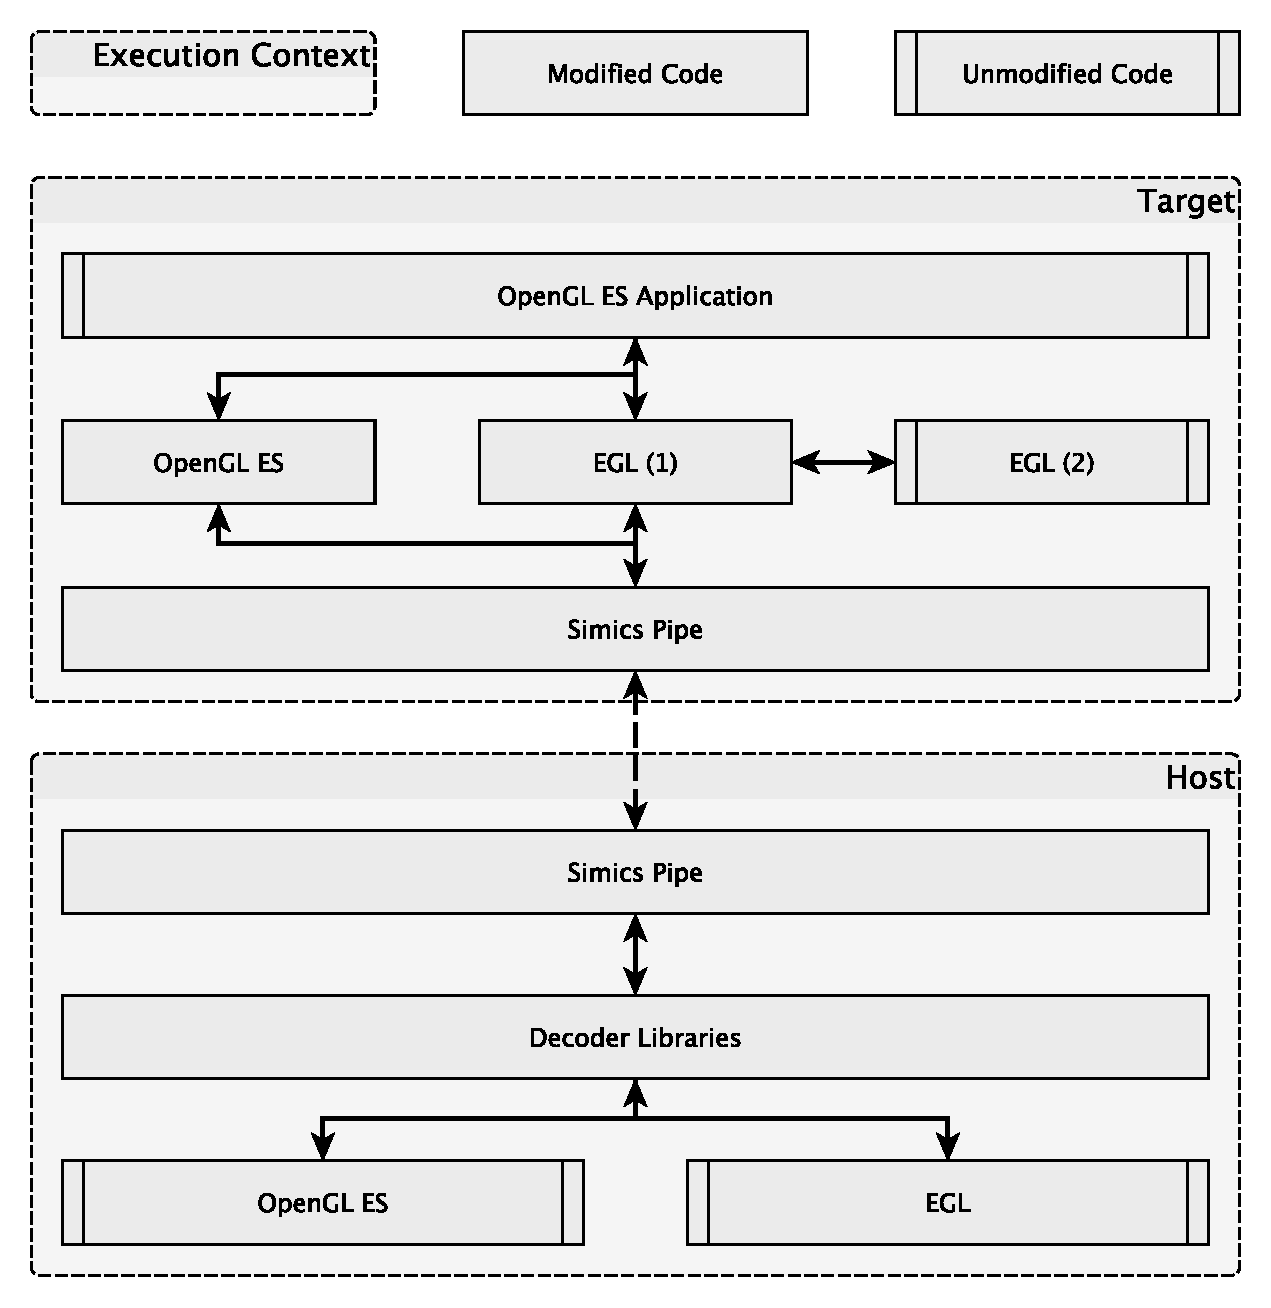
\includegraphics[width=\linewidth]{img/yedoverview.pdf}
\caption{Overview of paravirtualized graphics in Simics.}
\label{fig:overview}
\end{figure}

% Problem Formulation
\section{Problem Formulation}
\label{sec:problemformulation}
In regards to previous work in the area, there is no indication -- in academic writing -- of existing paravirtualized graphics in a simulator with advanced capabilities like Simics, featuring deterministic execution, checkpointing and reverse execution.
Potential performance gains on such a platform are inherently unclear due to these features, and accordingly incentivize a performance evaluation.
Such functionality could simplify debugging, testing, and profiling of applications comprising some GPU-bound workload, leveraging the benefits of using Simics for software and systems development with applications requiring graphics acceleration, e.g. responsive UIs.

As portrayed in Section~\ref{sec:previousresearch}, VMGL is an OpenGL virtualization solution for WMware Workstation and Xen platforms.
Based on conclusions drawn from VMGL, Lagar-Cavilla et al. concludes that target to host communications could be a potential performance bottleneck when using network communications.
Thus, as an alternative to network communications, Lagar-Cavilla et al. suggests utilizing a shared memory model, suspecting that such a paradigm might relieve any communications bottleneck.
Accordingly, this paper presents an OpenGL paravirtualization model using magic instructions to share VM memory directly from a simulated RAM image.

Entailed by these research gaps, the research questions formulated in this section are considered to be lacking in the field.

This paper presents the paravirtualization of OpenGL~ES~$2.0$ in the Simics full-system simulator. 
The study concerns investigating the performance of paravirtualized graphics in a modern virtual platform.
This entails development and analysis of efficient communication and execution in the Simics run-time environment.
The objectives of the paper is to evaluate the feasibility of paravirtualization as an approach to accelerate graphics in virtual platforms, and to identify the strengths and weaknesses of using magic instructions as a transparent communications bridge.

To accommodate the analysis of benefits and drawbacks of paravirtualized graphics, two benchmarks are devised.
The benchmarks are designed to stress latency in target-to-host communication and computational intensity brought on by complex GPU workloads.
As such, the purposes of these benchmarks is to stress a suspected bottleneck in the communication between target and host systems, and to measure how well the solution performs under computational stress.
The performance of these benchmarks is compared to that of traditional software rasterization.

Thus, this study is relevant to the field of computer science by expanding upon the the knowledge of graphics acceleration in virtual platforms.
Graphics acceleration in a virtual platform is relevant because it facilitates debugging, testing, and profiling of software which depends on GPU graphics acceleration.
By these means, this paper contributes to the field of computer science by answering these questions from the perspective of graphics paravirtualization in the Simics full-system simulator.
Formally, the paper seeks to answer the following research questions:

\begin{enumerate}
  \item What constitutes a viable implementation of paravirtualized graphics?
  \item What are the benefits and disadvantages of paravirtualized graphics?
  \item How does paravirtualized graphics performance relate to software rasterization?
\end{enumerate}
